\documentclass[a4paper, dutch, parskip=full]{scrartcl}
\usepackage[dutch]{babel}
\usepackage{graphicx}
\graphicspath{{./}}

\begin{document}

\title{ER diagram}
\author{}
\date{\today}
\maketitle
Nu volgen enkele extra notieties voor het ER schema.
\begin{itemize}
  \item Een mens in de database moet of een artiest of een designer zijn.
  \item Als een uitgever (publisher) n versies uitgeeft dan geeft hij maximaal n spellen uit.
  \item Een versie kan minimaal door nul verkopers worden verkocht, in het geval dat het ooit werd verkocht, maar nu niet meer.
  \item Fysieke verkopers en digitale verkopers in de ISA-hierarchie zijn `covering' en `disjoint'.
\end{itemize}

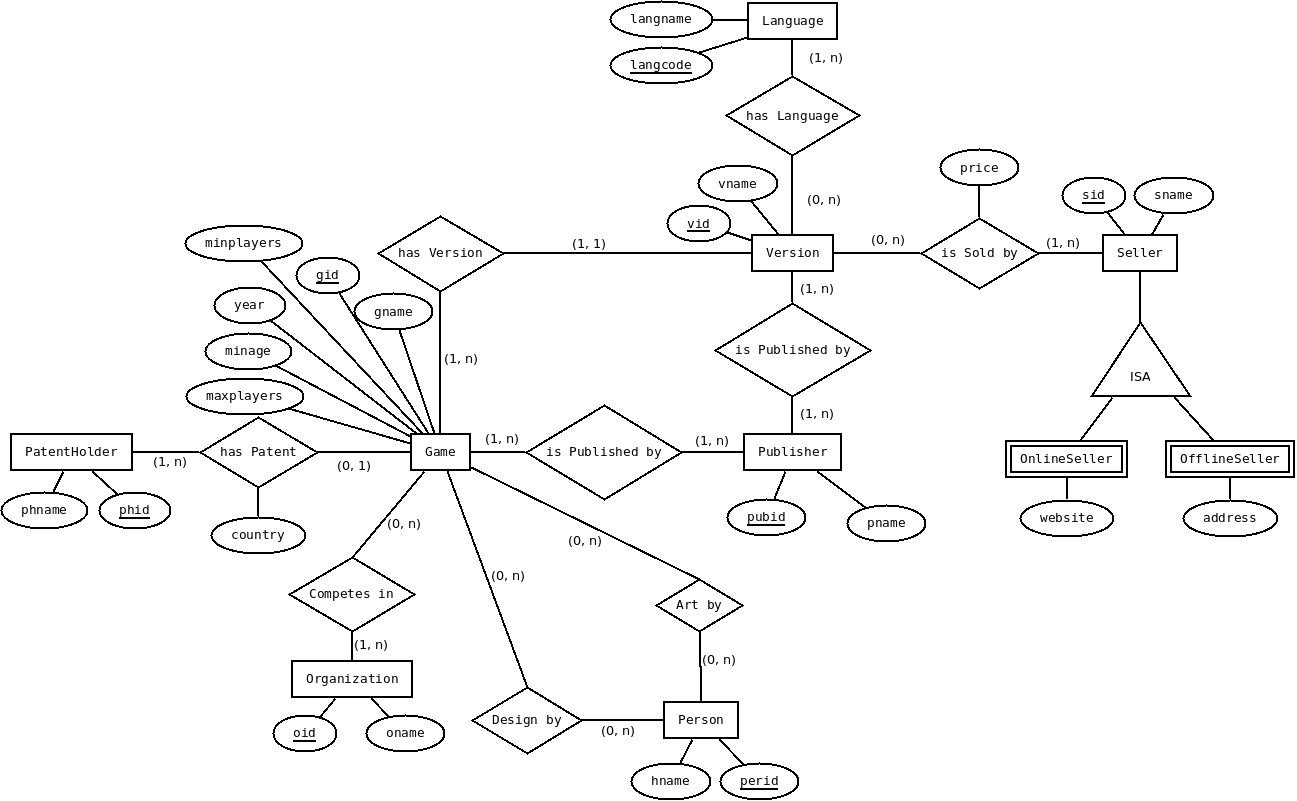
\includegraphics[scale=0.33]{ER}

\end{document}
